\documentclass[12pt,a4paper]{article}

\usepackage[utf8]{inputenc}
\usepackage[T1]{fontenc}
\usepackage{amsmath}
\usepackage{amssymb}
\usepackage{makeidx}
\usepackage{graphicx}
\usepackage{float}
\usepackage[width=17.00cm, height=24.00cm]{geometry}
\usepackage[polish]{babel}

\usepackage{hyperref}
\usepackage{listings}
\usepackage{color}

\renewcommand\lstlistingname{Quelltext}

\lstset{ % General setup for the package
	language=Python,
	basicstyle=\small\sffamily,
	numbers=left,
	numberstyle=\tiny,
	frame=tb,
	tabsize=4,
	columns=fixed,
	showstringspaces=false,
	showtabs=false,
	keepspaces,
	commentstyle=\color{red},
	keywordstyle=\color{blue}
}




\begin{document}


\tableofcontents

\section{Wstęp}
W ramach projektu każdy z naszej trójki miał wymysleć pomysł optymalizacji który można by zaimplementować w ramach zajęć oraz rozwiązać implementując jeden z algorytmów optymalizacyjnych.

\begin{itemize}
	\item Pomysł Dawida zakładał optymalizacje wydatków związanych z zakupem opału w sezonie grzewczym
	\item Pomysł Piotrka opierał się na optymalizacji zysków z hodowli roślinnej w średnim gospodarstwie rolnym.
	\item Pomysł Bartka bazował na maxymalizacji jakości komponentów w składanym komputerze przy minimalizacji kosztów
\end{itemize} 

Wspólną decyzją był pomysł Piotrka optymalizacji gospodarstwa rolnego.

\section{Model matematyczny}

	\subsection{Opis problemu:}
	Problem polega na stworzeniu kilkuletniego planu upraw dla niewielkiego gospodarstwa rolnego w zależności od zmiennej kategorii) jakości gleby (w postaci cyfry w zakresie od 0 - 100) i  odległości uprawy od gospodarstwa. Celem będzie maksymalizacja zysków . Zakładamy przy tym że co roku nabywamy nowy materiał siewny.

	\subsubsection{Stałe:}
	\begin{itemize}
		\item N - Liczba dostępnych pól uprawnych.
		
		\item Y - liczba lat planowania upraw.
		
		\item T - stały koszt dojazdu na kilometr
		
		\item P - powierzchnia pola uprawnego w hektarach (każde pole ma identyczną powierzchnię)
		
		\item $ D_i $ -  Odległość i-tego pola od gospodarstwa, gdzie i = 1,...,N
		
		\item $ C_x $ - koszt produkcji danej rośliny na jeden hektar (koszt materiału siewnego, koszt pracy ludzkiej, itp.), gdzie x - nazwa rośliny
		
		\item $ W_x $- wpływ uprawy na glebę (zależne od uprawianej rośliny)
		
		\item $ S_x $ - zsumowana ilość dopłat i  wszelkich dodatków (w zależności od uprawianej rośliny)
		
		\item $ G = [g_{qx}] $ - macierz zysków z pola gdzie komórka  $ g_{qx} $ zawiera zysk z danej rośliny w zależnie od jakości gleby q i uprawianej rośliny $ x $.
	\end{itemize}

	\subsubsection{Zmienne:}
	\begin{itemize}
		\item $y$ - Obecny rok, y = 1,...,Y
		
		\item $ Q = [ q_{yi} ]_{Y \times N} $ -  Macierz klas jakości gleby gdzie komórka $ q_{yi} $ zawiera jakość ziemi którą na i-tym polu w roku y.
	\end{itemize}
	
	\subsubsection{Postać rozwiązania:} 
	\begin{itemize}
		\item $ X = [x_{yi}]_{Y \times N} $ - macierz decyzyjna o wymiarach $ Y \times N $, gdzie komórka $ x_{yi} $ zawiera indeks rośliny którą siejemy na i-tym polu w roku y.
	\end{itemize}
	
	\subsubsection{Postać funkcji celu:}
	\begin{flalign}
		f(X) = \sum_{y=1}^{Y} \sum_{i=1}^{N} G_{q_{yi} x_{yi}} + S_{x_{yi}} - (C_{x_{yi}} * P + D_i * T)
		\\q_{yi} = q_{(y-1)i} + W_{x_{(y-1)i}}
	\end{flalign}  
	
	\subsubsection{Ograniczenia:}
	\begin{itemize}
		\item $ 0 \leq q_{yi} \leq 100 $ Jakość gleby może zmieniać się w zakresie od 0 do 100
		\item $ x_{i-1} \neq x_i $, gdzie $ x_k $ nie jest stanem pustym pola 
	\end{itemize}	


\section{Implementacja}
Naszą implementację zaczeliśmy od zaimplementowania modelu matematycznego w formie funkcji pythonowej. 

\label{postac_rozw}
Postać rozwiązania jest przedstawiana w postaci macierzowej (listy list w pythonie), gdzie wiersze przedstawiają lata symulacji zaś numery kolumn odpowiadają odpowiedniemu polu.

Funkcja celu matematycznie jest zapisana w formie podwójnej sumy, zaś zaprogramowana jako podwójna pętla for.
W programie nie jest to oczywiste ponieważ pętla po latach uprawy wywołuje w sobie funkcję pomocniczą w której jest kolejna pętla już idąca po polach.

\subsection{Implementacja klasy jako modelu rozwiązania}
Początkowo zakładaliśmy że cały nasz projekt będzie w postaci jednej klasy Pythona
jednakże w trakcie rozwiązywania problemu doszliśmy do wniosków że chcielibyśmy porównać dwa sposoby rozwiązania problemu dlatego też w pierwotnej klasie ... !TODO

\subsection{symulowane wyżarzanie}
Nasz problem, na podstawie sugestii pani Profesor postanowiliśmy rozwiązać algorytmem symulowanego wyżarzania (z ang. simulated anealling). Jest to nasz pierwszy pomysł na rozwiązanie problemu, w dalszej części opisujemy drugi, który jest zaimplementowany na podstawie metaheurystyki algorytmu genetycznego (z ang. genetic alg.).

\subsubsection{metody algorytmu}
Aby zaimplementować nasze rozwiązanie metaheurystyką symulowanego wyżarzania potrzebowaliśmy zdefiniować następujące funkcje: 

\begin{itemize}
	\item \begin{verbatim}
		simulated_annealing	
	\end{verbatim}
	
	\item \begin{verbatim}
		__annealing_temp
	\end{verbatim}

	\item \begin{verbatim}
		__annealing_neig
	\end{verbatim}

	\item \begin{verbatim}
		__annealing_P
	\end{verbatim}

\end{itemize}

\paragraph{annealing temperature}
Funkcja wspomagająca algorytm symulowanego wyżarzania, zwraca temperaturę według wzoru 1 - (k + 1)/kmax (jeśli wyrażenie jest pozytywne) lub 1/kmax jezęli wzór zwraca wrtości negatywne.
Ten sposób wyliczania temperatury wydawał się najprostszy i najpraktyczniejszy do zaimplementowania.

\paragraph{annealing Probability}
Funkcja pomocnicza akceptująca następujące parametry: wartość f. celu dla obecnego rozwiązania, wartość f. celu dla nowego rozwiązania, obecną temperaturę. Funkcja wylicza prawdopodobieństwo przejścia do wybranego, nowego rozwiązania.
Jako że maksymalizujemy to funkcja zwraca 1 jeżeli nowe rozwiązanie ma wyższą wartość niż obecne, zaś w przeciwnym wypadku jest wyliczane według wzoru: $ exp( (-1)* (f - f_{new}) / temp ) $. 

\paragraph{annealing neighbour}
Funkcja pomocnicza wybierająca kandydata na nowe rozwiązanie. Kandydat jest macierzą (\hyperref[postac_rozw]{wyjaśnienie tutaj}) w której zmieniono w randomowy sposób jedną roślinę (randomowo dobieramy rok i pole, czyli pozycję w macierzy). Roślina na jaką zamieniamy to pole w macierzy wybieramy randomowo z listy roślin z wykluczeniem poprzedniej na tej pozycji.
Funkcja wykorzystuje model brute-force do sprawdzenia czy nowe rozwiązanie nadaje się do symulacji, tzn. czy nie wyskoczy żaden błąd przy próbie odpalenia simulate farm, zaś jeżeli wyskoczy rekurencyjne powtórzenie funkcji. 

	\paragraph{simulated annealing}
Główna funkcja zaimplementowanego algorytmu na podstawie pseudo-kodu:

\begin{figure}[H]
	\centering
	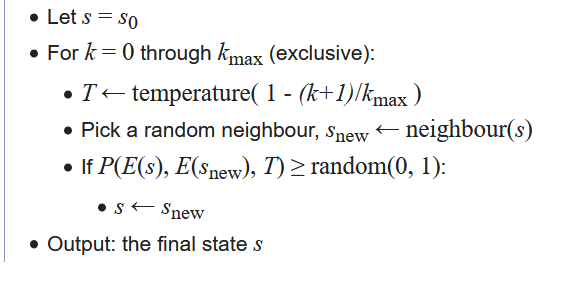
\includegraphics[width=1\linewidth]{screens/pseudocode}
	\caption{Pseudo-kod głównej części algorytmu simulated annealing}
	\label{fig:pseudocode}
\end{figure}


Algorytm działa $ k_{max} $ razy w pętli for, 
w pierwszym kroku każdej iteracji jest przypisywana nowa temperatura zwracana z funkcji annealling temp


\subsection{algorytm genetyczny}


\subsection{wyniki}





\section{Problemy}
Indeksacja

wybór następnego kandydata na rozwiązanie


	

\end{document}